This Exercise has been implemented in "Q0013.py".
\subsection{}
\subsection{}
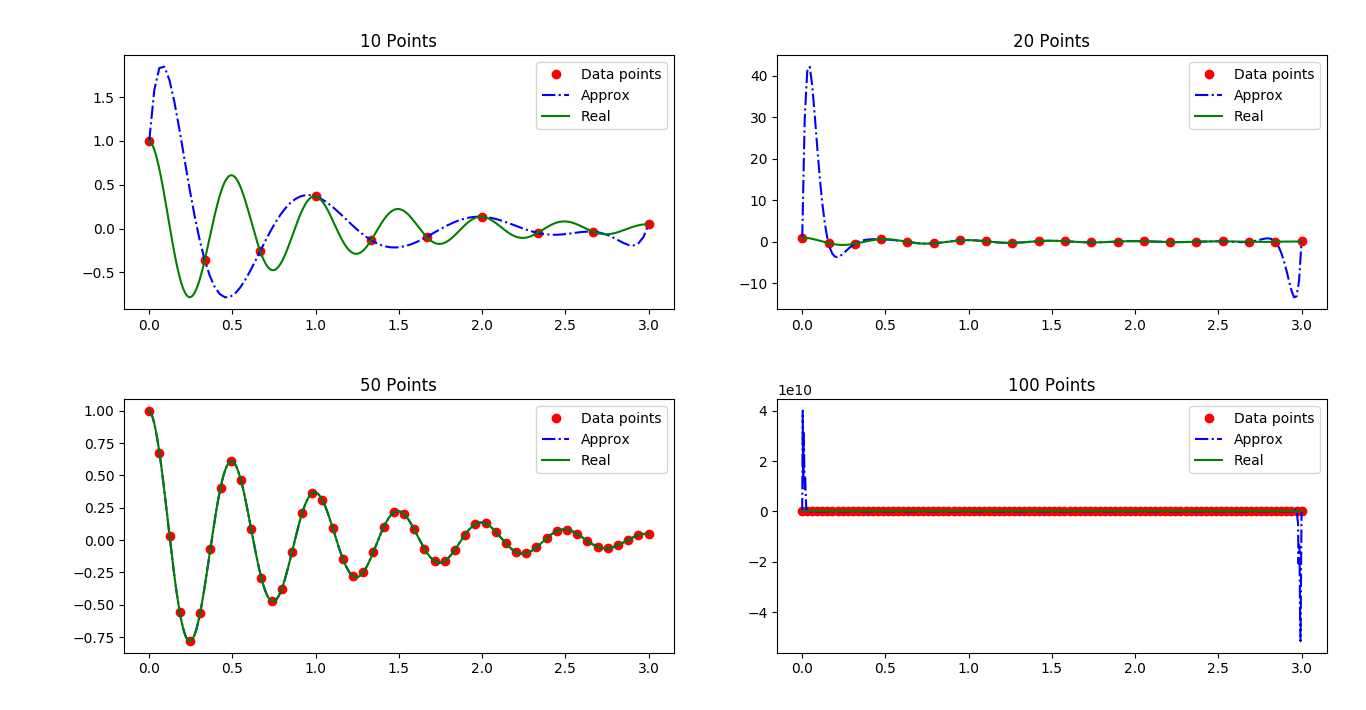
\includegraphics[width=\linewidth]{plots}
\subsection{}
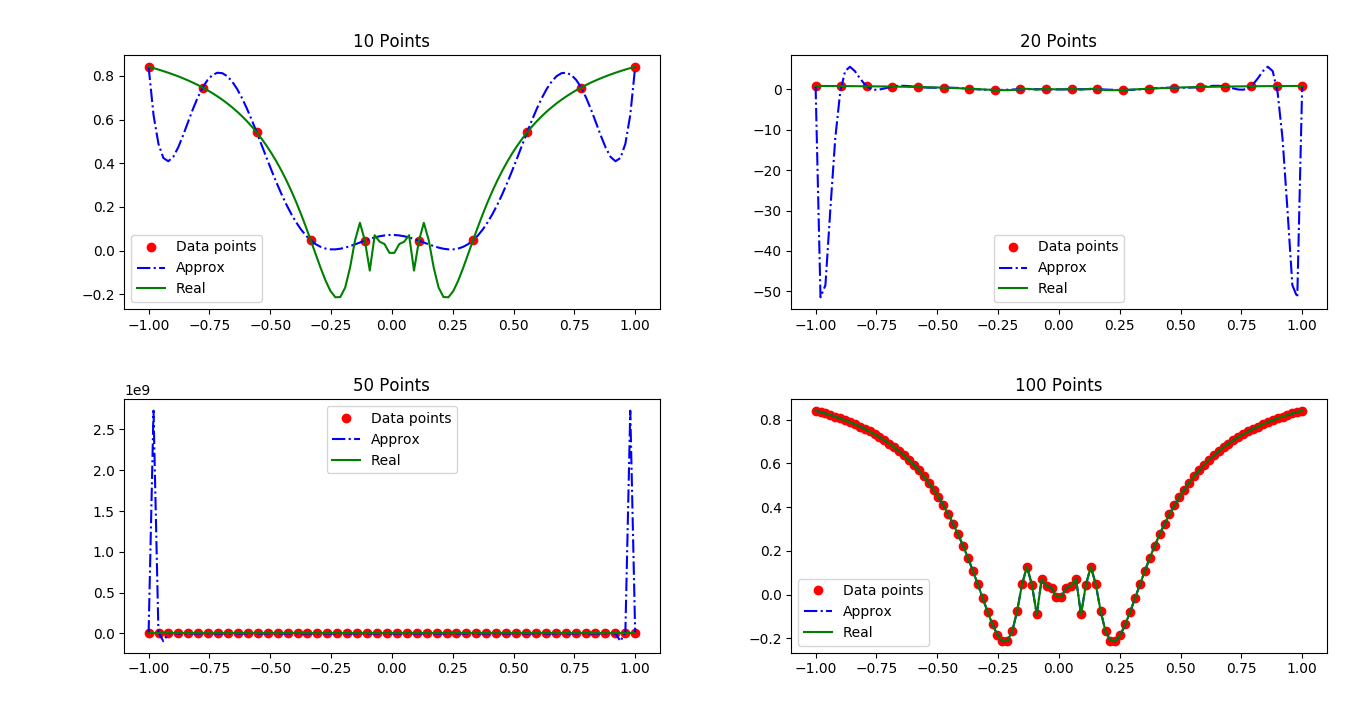
\includegraphics[width=\linewidth]{plots1}
The approximate functions have been plotted with 10 times as many points as there are data points in the corresponding plot, and the "real" functions have been plotted with 1000 points. It is interesting to note that as we use more and more data points to approximate the function, it becomes significantly more precise in the middling parts of the interval. However, at the outer edges of the interval, the imprecisions rise extremely quickly, with the approximate functions reaching extremely large values.
\subsection{}
We start by writing the function as per Theorem 6.1.2 in the book:
\begin{align*}
  |f(x) - p_n(x)| &= \frac{1}{(n+1)!} f^{n+1}(\mathcal{E}x)\prod^n_{i=0}(x-x_i)
\end{align*}
We start by finding an upper bound for $f^{n+1}(\mathcal{E}x)$, with the help of the general Leibniz rule:
\begin{align*}
  f^{n+1}(\mathcal{E}x) &= \left(\frac{d}{dt}\right)^{n+1} (e^{-t} cos(4\pi t)) \\
  &= \sum^{n+1}_{k=0} \begin{pmatrix} n+1 \\ k \end{pmatrix} \left(\frac{d}{dt}\right)^{(n+1-k)}(e^{-t}) \cdot \left(\frac{d}{dx}\right)^k cos(4\pi t)
\end{align*}
We can bound each of the derivative terms here:
\begin{align*}
  \left(\frac{d}{dt}\right)^{(n+1-k)}(e^{-t}) &\leq e^0 = 1 \\
  \left(\frac{d}{dx}\right)^k cos(4\pi t) &\leq 1 \cdot (4\pi)^k
\end{align*}
We insert this into $f^{n+1}(\mathcal{E}x)$:
\begin{align*}
  f^{n+1}(\mathcal{E}x) &\leq \sum^{n+1}_{k=0} \begin{pmatrix} n+1 \\ k \end{pmatrix} (4\pi)^k
\end{align*}
We can simplify this by using this expansion:
\begin{align*}
  \sum_{k=0}^n \begin{pmatrix} n \\ k \end{pmatrix} x^k &= (1 + x)^n \\
  \sum^{n+1}_{k=0} \begin{pmatrix} n+1 \\ k \end{pmatrix} (4\pi)^k &= (1 + 4\pi)^{n+1} \\
  f^{n+1}(\mathcal{E}x) &\leq (1 + 4\pi)^{n+1}
\end{align*}
Because $t \in [0,3]$, we can bound the following:
\begin{align*}
  \prod_{i=0}^n(x-x_i) \leq 3^n
\end{align*}
Thus, we have a bound on $|f(x) - p_n(x)|$:
\begin{align*}
  |f(x) - p_n(x)| &\leq \frac{3^n \cdot (1 + 4\pi)^{n+1}}{(n+1)!}
\end{align*}
